\documentclass[11pt]{article}
\usepackage[top=1.00in, bottom=1.0in, left=1in, right=1in]{geometry}
\renewcommand{\baselinestretch}{1.1}
\usepackage{graphicx}
\usepackage{natbib}
\usepackage{amsmath}
\usepackage{parskip}

\def\labelitemi{--}
\parindent=0pt

\begin{document}
\renewcommand{\refname}{\CHead{}}

{\bf Is photoperiod the dominant or least important cue for woody plant spring phenology?} % Or, is it both?

Woody plant leafout and flowering each spring is strongly driven by warm spring temperatures, and thus has shifted days to weeks earlier with anthropogenic climate change. But how long this advance can continue depends on the relative importance of the two other major environmental cues---chilling (via the accumulation of cool winter temperatures) and photoperiod. Over a decade of focused research \citep[e.g.,][]{laube2014gcb,ospreebbms} has found chilling produces the largest shifts in spring phenology, often 3-5X larger than the response to photoperiod \citep{morales2024phylogenetic}. But this research generally tests photoperiod responses in only one way (Fig. \ref{fig:waldedata}) that is disconnected from the molecular concept of critical photoperiod. At the same time, new studies suggest a dominating role of solstice mid-season phenology \citep{zohner2023effect,Journe2024}, and a remarkably stable photoperiod response across most species (Fig. \ref{fig:phylopheno}). Together these new results suggest an important and poorly understood role of photoperiod that may not be well tested by current methods.  Building a mechanistic predictive model of spring phenology thus requires re-examining how much we actually know currently and developing new approaches. 

\emph{Here, I want to explore:}
\begin{enumerate}
\item How do current findings in woody plant spring phenology experiments compare to our understanding of photoperiod from the molecular literature? Most studies manipulate photoperiod alongside forcing and chilling temperatures usually by using two different constant photoperiods with only small responses (Fig. \ref{fig:waldedata}). 
\item What experiments could help better understand mechanistically how photoperiod affects spring phenology?
\end{enumerate}

\emph{We have data on many woody plant spring phenology experiments and can explore:}
\begin{enumerate}
\item Differences in photoperiod responses for budburst versus flowering (since most molecular research is on flowering, right?).
\item Budburst \% versus timing responses to photoperiod.
\item Whether any studies do light interruption (I have not found any in our database of woody plant spring phenology, but I saw some for strawberry, which was included by accident). 
\item Compare findings we see from molecular experiments such as those that Stacey Harmer pointed out where the response is considered not important, but is actually just small compared to the larger responses seen usually to critical photoperiod. 
\end{enumerate}

\clearpage
\section*{References}
\bibliographystyle{/Users/Lizzie/Documents/EndnoteRelated/Bibtex/styles/besjournals}
\bibliography{/Users/Lizzie/Documents/git/bibtex/LizzieMainMinimal}

\section*{Figures}

\begin{figure}[h!]
\includegraphics[width=1\textwidth]{..//..//cherries/data/walde_etal/figures/waldehighchillphoto.pdf}
\caption{Results from Walde \emph{et al.} 2023 for budburst timing across species under high chilling and two photoperiods: 8 and 16 hours. This type of study is the most common type done in woody plant phenology---it uses cuttings of dormant buds exposed to chilling (cool temperatures) followed by different combinations of warm temperatures and photoperiods (this study is unique though in covering a wide range of forcing temperatures).} % walde.R
\label{fig:waldedata}
\end{figure}


\begin{figure}[h!]
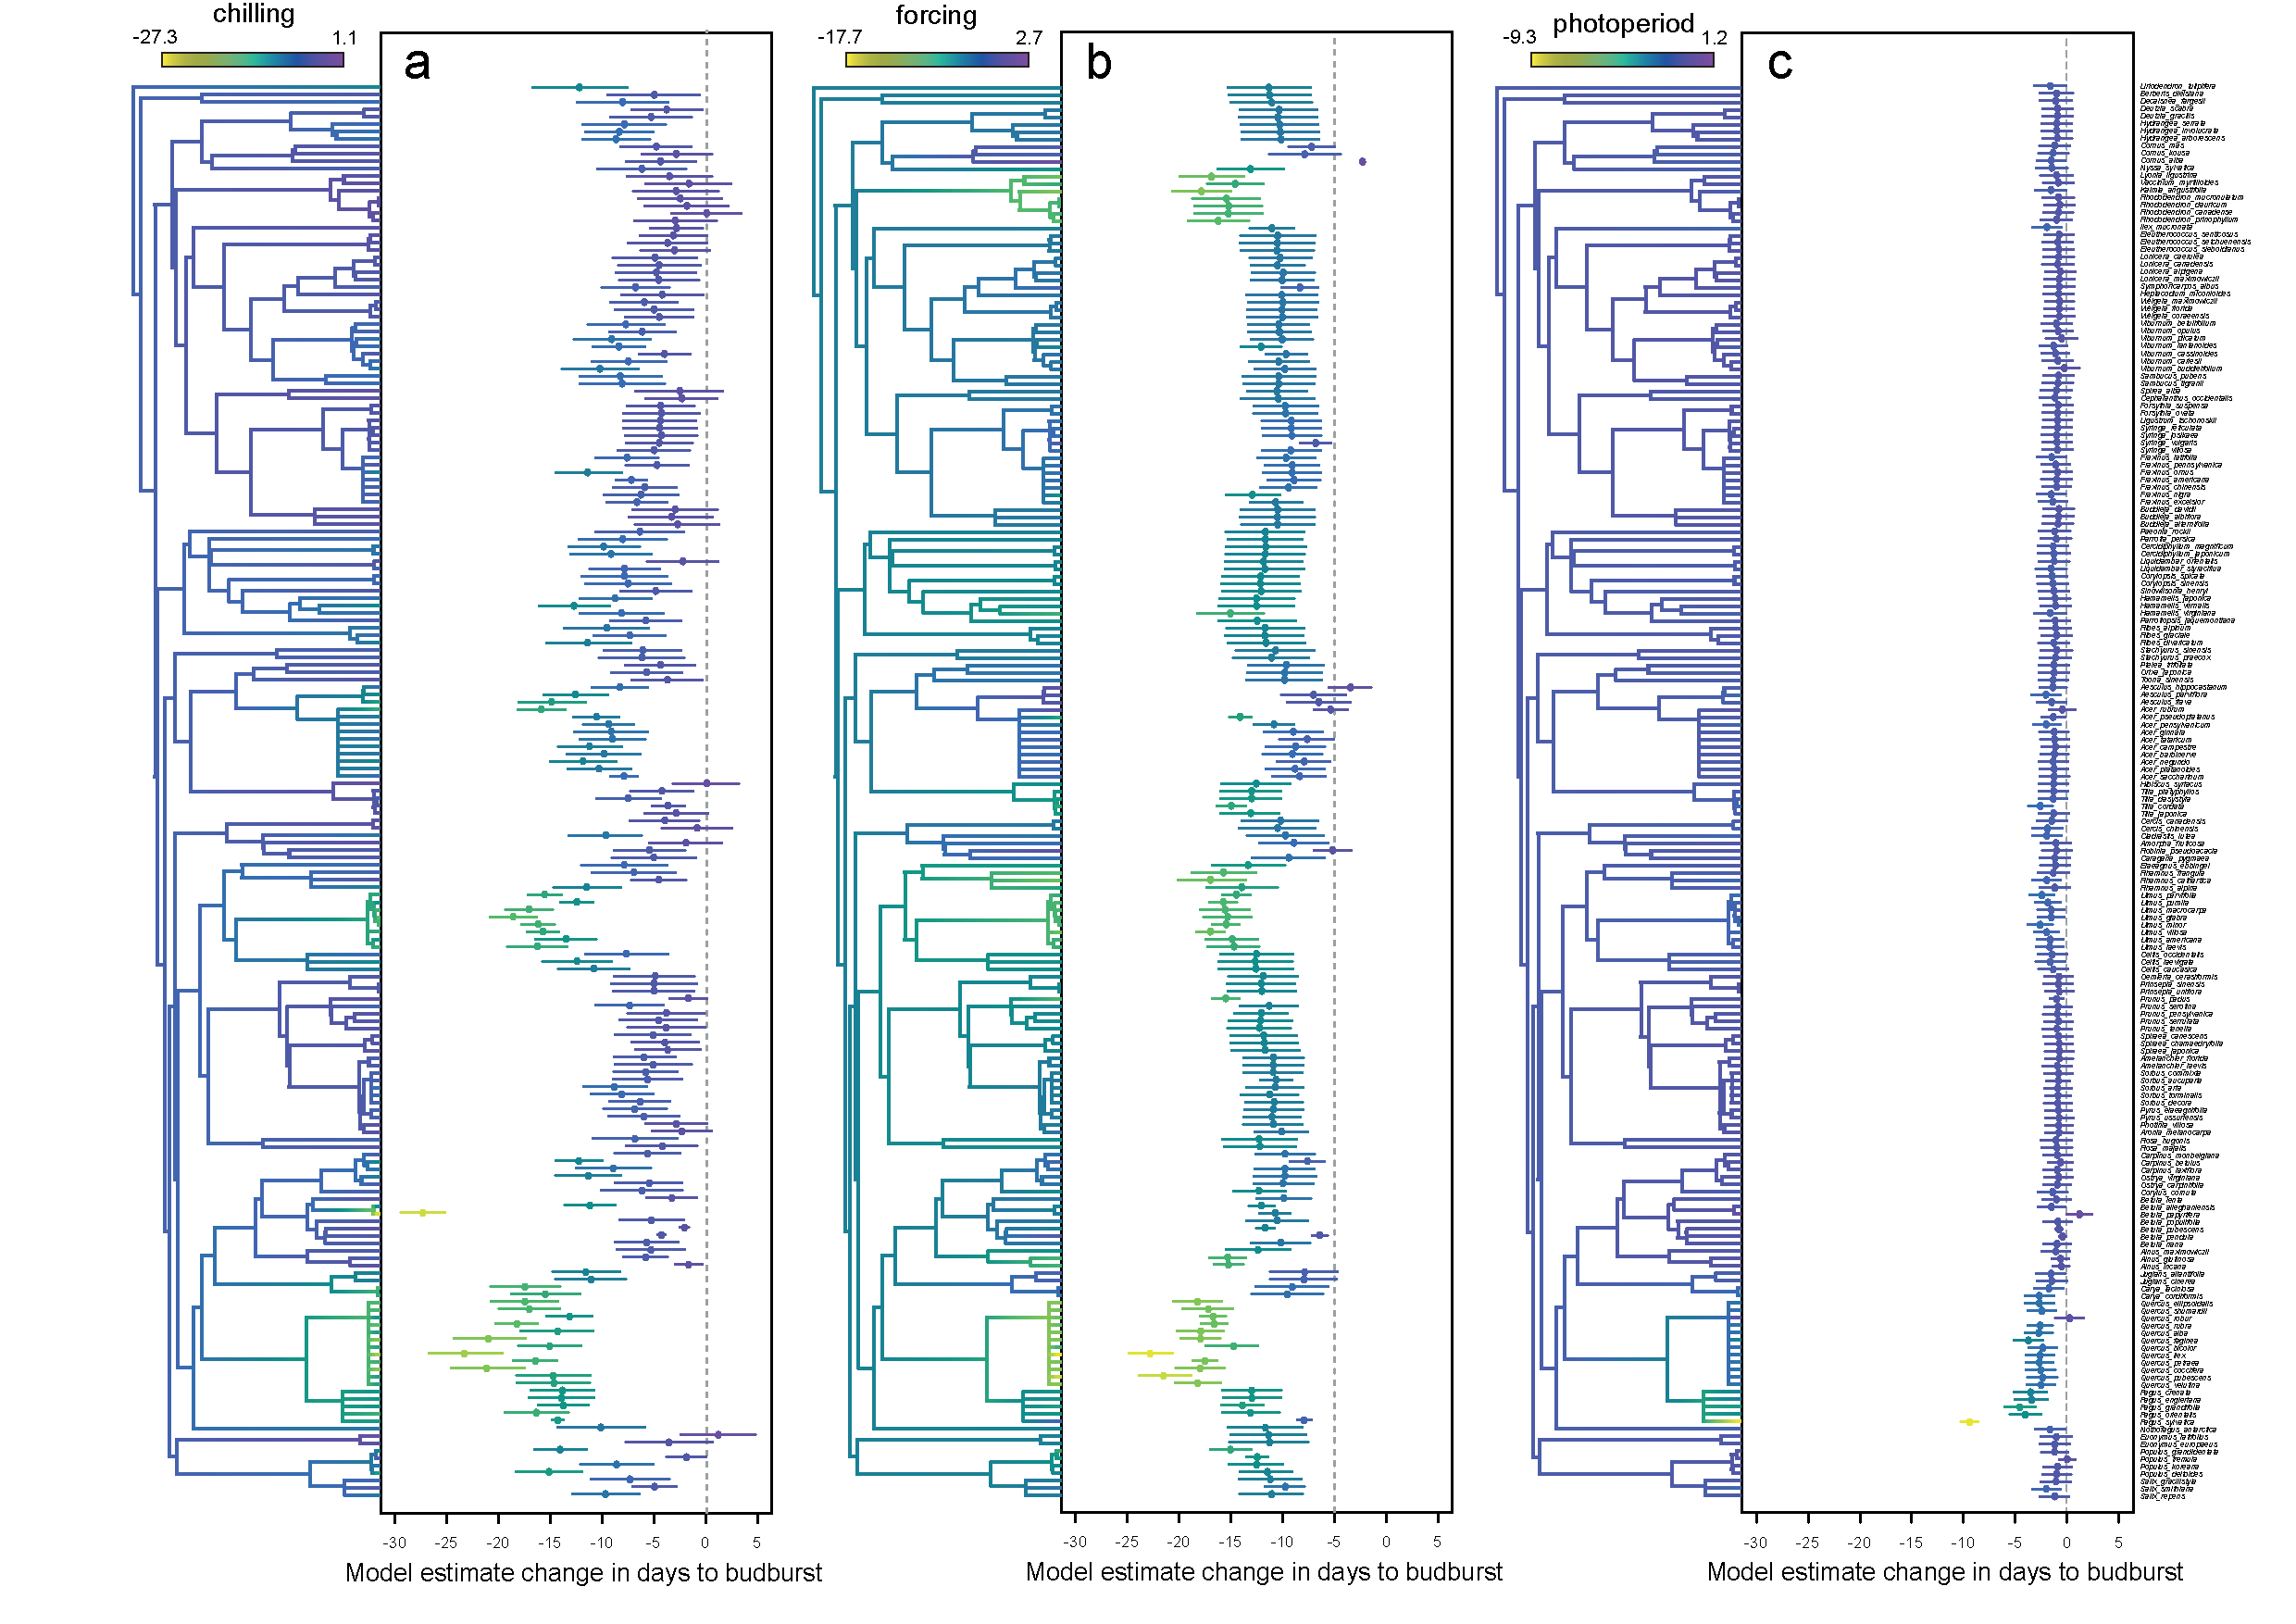
\includegraphics[width=1\textwidth]{..//figures/Fig1_phylo_muplots191.pdf}
\caption{Estimated chilling, forcing and photoperiod responses (in units standardized by the mean and SD for each response variable) from 191 woody angiosperm species show most species shift earlier two days per standardized photoperiod unit, except for \emph{Fagus} species with the well-studied \emph{Fagus sylvatica} showing the strongest response. Figure reproduced from \citet{morales2024phylogenetic}.} 
\label{fig:phylopheno}
\end{figure}


\end{document}

